\chapter{Heterogeneous Cooperative Spectrum Sensing (CSS)}
\label{chapter3}

This chapter provides the background information needed to understand the chapters that follows. It examines the basic outlines of a heterogeneous networks and how cooperative spectrum sensing (CSS) can help in enhancing the accuracy of signal source estimation. The fusion center (FC) collects the data from the sensor node network and process it to make the reliable decision. Secondly, this chapter investigates various algorithms which can be used in heterogeneous network to estimate signal source. Finally, it also outlines the necessary hardware and software tools used in the implementation of heterogeneous CSS chapter.

\section{Cognitive Radios}
Cognitive radio (CR)~\cite{cogjm} is a communication systems paradigm that focuses on employing highly agile, environmentally aware, intelligent wireless platforms in
order to autonomously select and configure device operating parameters based on the prevailing radio and network environmental conditions~\cite{bookhtn1}. In general the cognitive radio may be expected to look at parameters such as channel occupancy rate, available channels, bandwidth required for data transmission and the modulation types that may be used. It must also look at the regulatory requirements set by the Federal Communications Commission. In some instances a knowledge of geography and this may alter what it may be allowed to do. Software-defined radios (SDR) are mainly responsible for making cognitive radios used in wireless communications system a reality. Software radios provide a vast untapped potential to personalize services, and they make the process of modifying the radio characteristics extremely simple. 

The work is underway to determine the best possible methods of developing the cognitive radio communications system that can fulfill all its requirements. To facilitate the intelligent decision making capabilities in these cognitive radio systems, machine learning algorithms have been proposed in the literature~\cite{barker2008mission,haykin2005cognitive,newman2007cognitive,newman2008population} to automate the reconfiguration process. The Figure~\ref{cograd} describes the various building blocks of a cognitive radio system. The spectrum sensing is performed to estimate the spectrum holes in the band and after the analysis the decision strategy is prepared. The radio is configured with the new parameters based on the radio environment and the spectrum decision made.  

\begin{figure}[ht!]
	\centering
	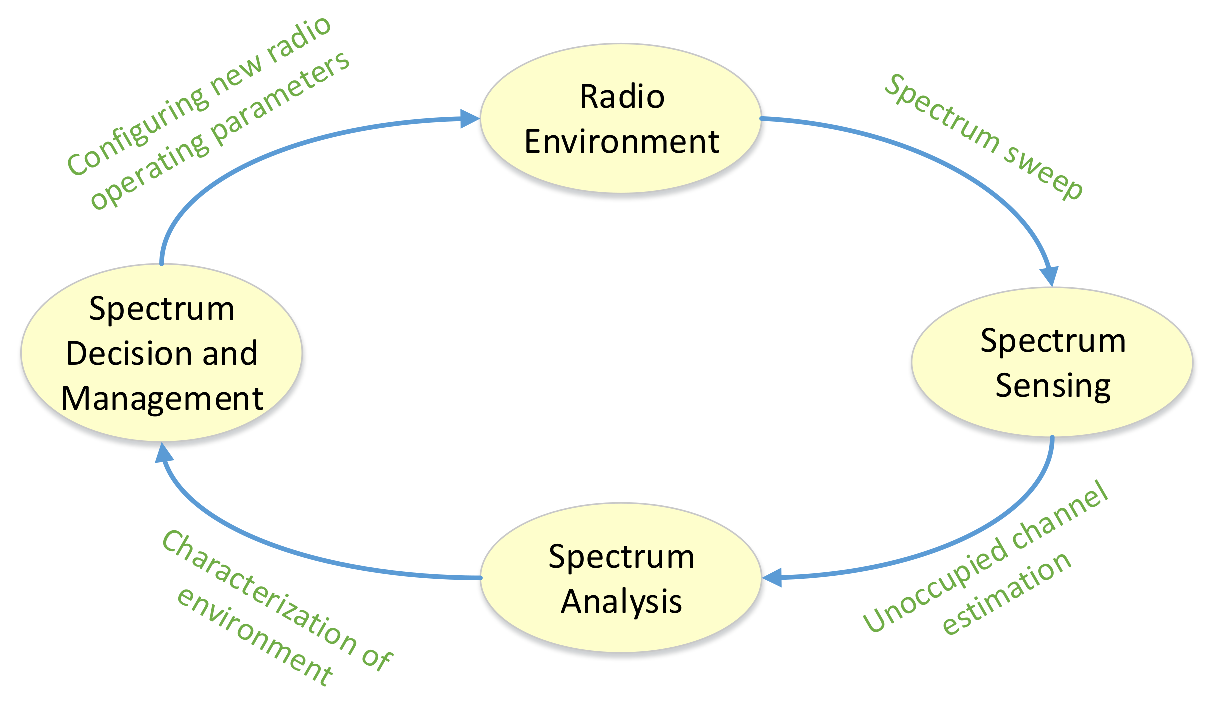
\includegraphics[width=\textwidth,keepaspectratio]{images/Gill/figs/cognitive_radio.eps}
    \caption{The block diagram explaining the basic parts of Cognitive Radio system. The operating parameters are configured based on the characterization of the wireless environment.} 
\label{cograd}      
\end{figure}

\section{Cooperative Spectrum Sensing in Heterogeneous Networks}
In Heterogeneous CR network, each radio is equipped with different numbers of antennas, sampling rates and RF characteristics. In addition, each sensor node may experience distinct channel fading and suffer from different noise levels due to their respective locations and device performances, such as amplifier and ADC.  As a result, each node may have different sensing capabilities and reliability values. This is a universal and fundamental characteristic of a heterogeneous CR network which requires robust algorithms to achieve high accuracy in signal source detection for estimating the presence of a primary user\cite{arhtn13}. In this thesis, we investigate the cooperative spectrum sensing in heterogeneous networks with a centralized FC, a transmitter acting as a signal source and four sensor nodes. As explained earlier we are using energy detection as one of the spectrum sensing technique since it possesses a very low implementation complexity~\cite{arhtn4}. The energy detection scheme detects the presence or absence of a signal source based on its intercepted energy signature. If the energy of the signal is higher than a certain threshold, this indicates that the channel is occupied. The ED can be modeled by the equation:
\begin{equation}
	\label{eq:1}
     y(n) = 
     \left\{
     \begin{aligned}
   &w(n),~~~~~~~~~\Hmat_0\\
   &s(n) + w(n),~\Hmat_1
    \end{aligned}
    \right.
\end{equation}
where $y(n)$ represents the received signal, $s(n)$ represents the signal source PU, and $w(n)$ is the white Gaussian noise $w(n) \sim N(0,\sigma_n^2) $. $\Hmat_0$ describes the hypothesis when there is no signal present, while the hypothesis $\Hmat_1$ is the presence of signal.

The decision whether the signal is present or absent is decided by evaluating a local test statistic $L$ to see whether it is above or below certain fixed threshold $\tau$. 
The local test statistic $L$, which is the complex-magnitude squared of the FFT samples, is compared with $\tau$ using equation:

\begin{equation}
\label{eq:2}
	L = \sum_{n=1}^{M}{|y(n)|^2} = 
	\left\{
	\begin{aligned}
		<\tau,~\Hmat_0 \\
		>\tau,~\Hmat_1		
	\end{aligned}
	\right.
\end{equation}

where $|y(n)|^2$ is the energy of a specific FFT bin and n=1,2,3...M are the number of samples received.

The probability of false alarm $P_{fa}$ and probability of detection $P_d$ are given by:
\begin{equation}
\label{eq:3}
P_f = Q\Bigg(\dfrac{\tau-M(2\sigma_n^2)}{\sqrt{M}(2\sigma_n^2)}\Bigg),
\end{equation}

\begin{equation}
\label{eq:4}
~~~~~~~P_d = Q\Bigg(\dfrac{\tau-M(2\sigma_n^2)(1+\gamma)}{\sqrt{M(1+2\gamma)}(2\sigma_n^2)}\Bigg).
\end{equation}
In cooperative spectrum sensing, each sensor node transmits the local sensing data to the fusion center for signal source detection. The local sensing data has to be quantized, thus yielding quantization errors. To minimize the quantization error in local test statistic $L$ and to reduce the effect of noise variance, the energy of the received signal $y(n)$ is normalized\cite{arhtn13}. The local test statistic $L$ for the $r^{th}$ sensor node is given as:
\begin{equation}
	\label{eq:5}
	L_r = \dfrac{1}{M_r\sigma_{n,r}^2}\sum_{r=1}^{M_r}|y(n)|^2
\end{equation}
where $M_r$ is the number of samples used to estimate the power of the signal source in the node,  $\sigma_{n,r}$ is the noise power variance.

In Eq~(\ref{eq:1}) $s(n)$ is considered as a deterministic signal and $w(n)$ is a Gaussian random variable with a variance of $\sigma_n^2$. Based on CLT, $L_r$ will have a following distribution~\cite{inphtn7}:

\begin{equation}
	\label{eq:6}
	L_r = 
	\left\{
	\begin{aligned}
		& N(1,\dfrac{1}{M_r}),~~~~~~~~~~~~\Hmat_0 \\
		& N(\gamma_r+1,\dfrac{1+2\gamma_r}{M_r}),~\Hmat_1		
	\end{aligned}
	\right.
\end{equation}
where $\gamma_r$ is the received SNR of the $r^{th}$ SU. The local decision statistic $L_r$ is quantized before transmission due to the bandwidth constraint, and this can lead to quantization errors. The values of $L_r$ received by FC can be modeled as:
\begin{equation}
	\label{eq:7}
	 \beta_r = L_r + w_{q,r},
\end{equation}
where $\beta_r$ is the decision statistic received by the FC and $w_q$ is the noise added to the signal due to fading and quantization error. In \cite{arhtn14}, the $w_q$ is modeled as a Gaussian noise with zero mean and $\sigma_q^2$ variance.

\section{Software Defined Radios}
We have already explained about the cooperative spectrum sensing in heterogeneous networks, now in this section we will look at the platform for testing the CSS algorithms. The platform which we use is a new hardware frontier called Software-Defined Radio (SDR) and is discussed in details.

\begin{figure}[ht!]
	\centering
	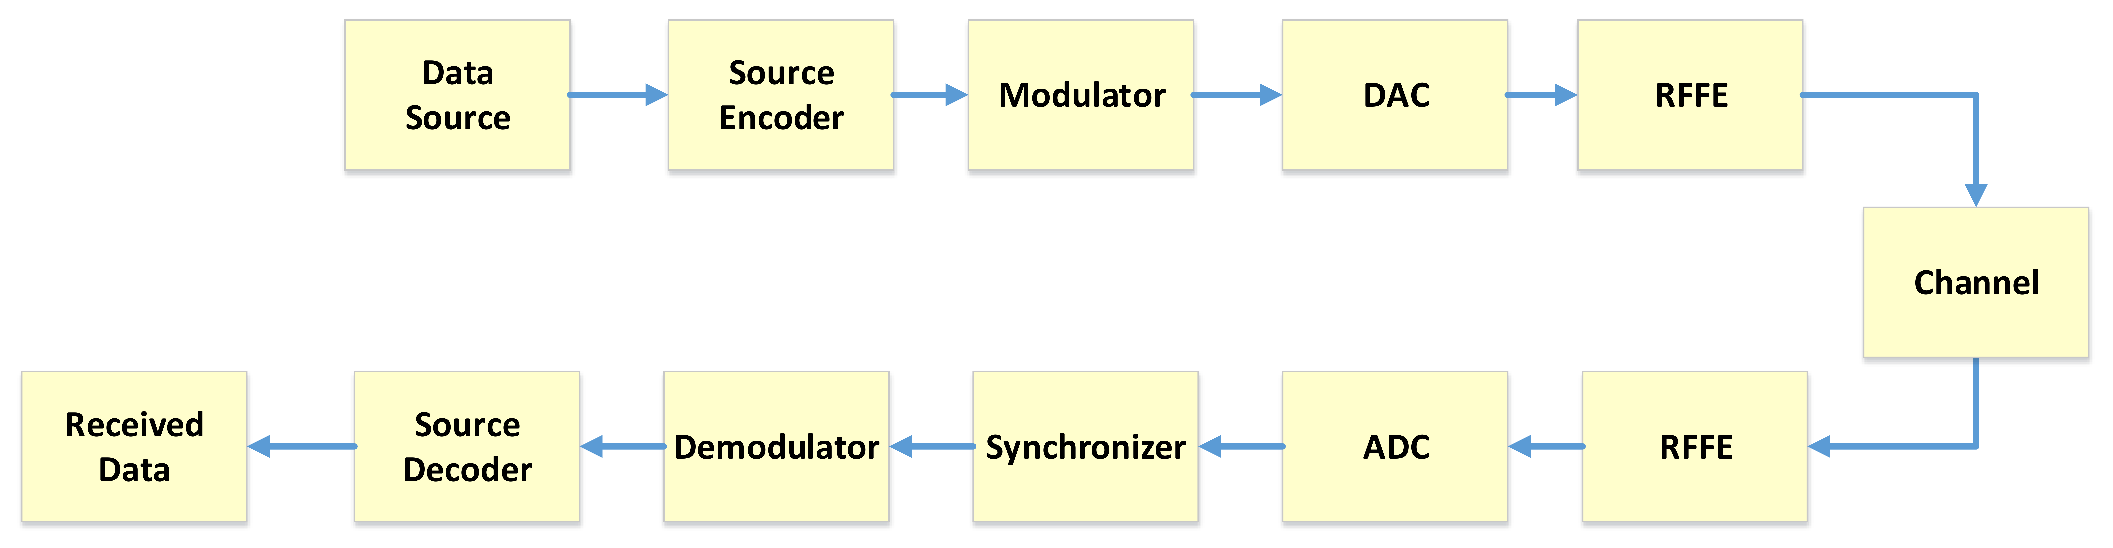
\includegraphics[width=\textwidth,keepaspectratio]{images/Gill/figs/softwaredefinedradio.eps}
    \caption{Software defined radio pushes all the adaptive elements and data manipulation operation into software. The goal of SDR is to provide or define all of the radio operation in software.} 
\label{sdr}      
\end{figure}

There has been a huge shift in the definition of a Software-Defined Radio and it has a lot to do with the question of where the hardware ends and software begins. Dr. J. Mitola III coined the Software Defined Radio which he described as a of digital signal processing (DSP) primitives, a meta-level system for combining the primitives into communication system (Tx, channel model, Rx, etc.), functions and a set of target processors on which the software radio is hosted for real-time communications~\cite{267870}. Dr. J. Mitola explains in the paper how software provides the flexibility which using hardware alone can never be achieved. And as time progresses SDR would become more dominant and close to ideal Cognitive Radio system.

The SDR technology existed since the 1970s but the key milestone in the advancement of SDR technology took place in early 1990s with the U.S. military initiative called SpeakEasy I/II. The SpeakEasy project was implemented to use programmable processing to emulate more than ten existing military radios, operating in frequency bands between 2 MHz and 2 GHz~\cite{392998}. With SpeakEasy the operator could talk to ten radios operating under different standards with any hardware modifications. With all these features, unfortunately there were some shortcomings which left much to be desired. The device was large enough to fit on the back of a pickup truck~\cite{392998} which is good for ground station but not if the mobility is an important factor. And in 1992 the field programmable gate arrays (FPGA) were not computationally efficient, hence required large time to change their operating characteristics. The two software-defined radios we used in the thesis are Universal Software Radio Peripheral (USRP N210) and RTL-SDR R2832U. In the subsequent subsections we discuss the two SDRs in detail.

\subsection{Universal Software Radio Peripheral (USRP) N21	0}

The USRP N210 has a very different RF characteristics compared to RTL-SDR hence modeling an ideal heterogeneous network. The USRP N210 provides a very high bandwidth, dynamic range processing capability. The product architecture includes a Xilinx Spartan 3A-DSP 3400 FPGA~\cite{xilinx}, 100 MS/s dual ADC, 400 MS/s dual DAC and gigabit ethernet connectivity to stream data to and from host processors. A modular design allows the USRP N210 to operate from DC to 6 GHz, while an expansion port allows multiple USRP N210 series devices to be synchronized and used in a MIMO configuration. 

\begin{figure}[ht!]
	\centering
	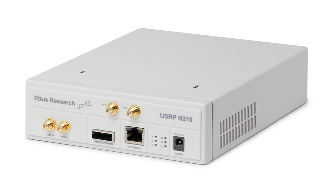
\includegraphics[width=0.75\textwidth,keepaspectratio]{images/Gill/figs/usrp.eps}
    \caption{USRP N210.} 
\label{usrp}      
\end{figure}

An optional GPSDO module can also be used to discipline the USRP N210 reference clock to within 0.01 ppm of the worldwide GPS standard. The USRP N210 can stream up to 50 MS/s to and from host applications. Users can implement custom functions in the FPGA fabric, or in the on-board 32-bit RISC softcore. The USRP N210 provides a larger FPGA than the USRP N200 for applications demanding additional logic, memory and DSP resources. The FPGA also offers the potential to process up to 100 MS/s in both the transmit and receive directions. The FPGA firmware can be reloaded through the Gigabit Ethernet interface~\cite{usrp}.

\subsection{RTL-SDR Software-Defined Radio}
RTL-SDR is a very cheap software defined radio that uses a DVB-T TV tuner dongle based on the RTL2832U chipset. With the combined efforts of Antti Palosaari, Eric Fry and Osmocom it was found that the signal I/Q data could be accessed directly, which allowed the DVB-T TV tuner to be converted into a wideband software defined radio via a new software driver.

\begin{figure}[ht!]
	\centering
	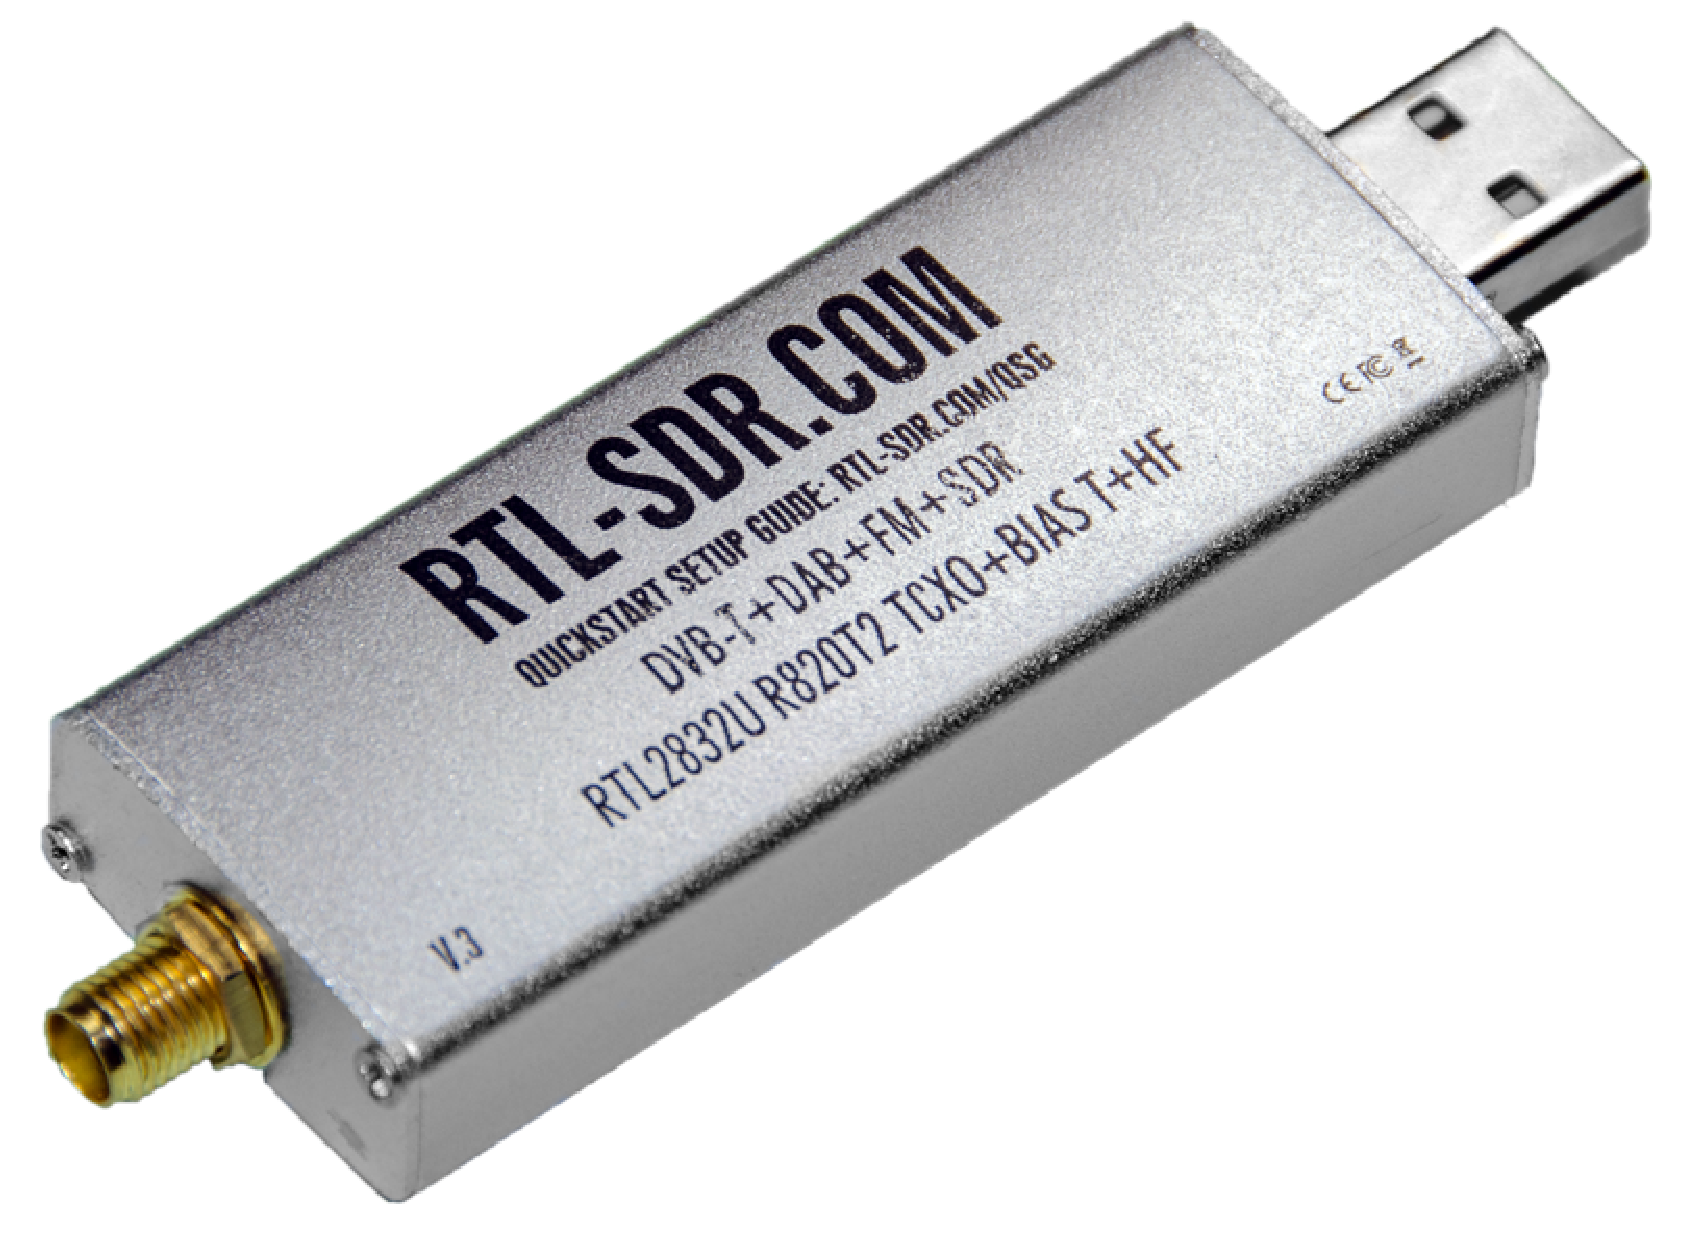
\includegraphics[width=0.75\textwidth,keepaspectratio]{images/Gill/figs/rtlsdr.eps}
    \caption{RTL-SDR R2832u} 
\label{rtlsdr}      
\end{figure}

Essentially, this means that a cheap \$20 TV tuner USB dongle with the RTL2832U chip can be used as a computer based radio scanner. This sort of scanner capability would have cost hundreds or even thousands of dollars just a few years ago. The RTL-SDR is also often referred to as RTL2832U, DVB-T SDR, RTL dongle or the “\$20 Software Defined Radio”.

\subsection{GNURadio and Software-Defined Radio}
The first software package to be discussed by this thesis is GNU Radio. GNU Radio provides the reconfigurable signal processing blocks that are necessary for software defined
radios. GNU Radio is an open source project allowing for SDR developers to develop unique signal processing blocks and SDR systems. GNU Radio was started in 2001, originally
forked from the SpectrumWare project developed at the Massachusetts Institute of Technology [46]. Since 2001, the code base has undergone massive changes, containing almost
no code from the original SpectrumWare project. Physically the code consist of three languages Python, C++, and SWIG. Python provides the overarching control of the system or
program, while C++ provides the actual signal processing blocks and mathematics. SWIG is a wrapper for C++ which allows Python to dynamically wrap around C++ and control
or compile with it. A diagram below better illustrates this architecture. It is also important to mention that there as significant paradigm shifts in the community, pushing more and more code to Python rather than C++, due to its easier programming syntax and structure.

\begin{figure}[ht!]
	\centering
	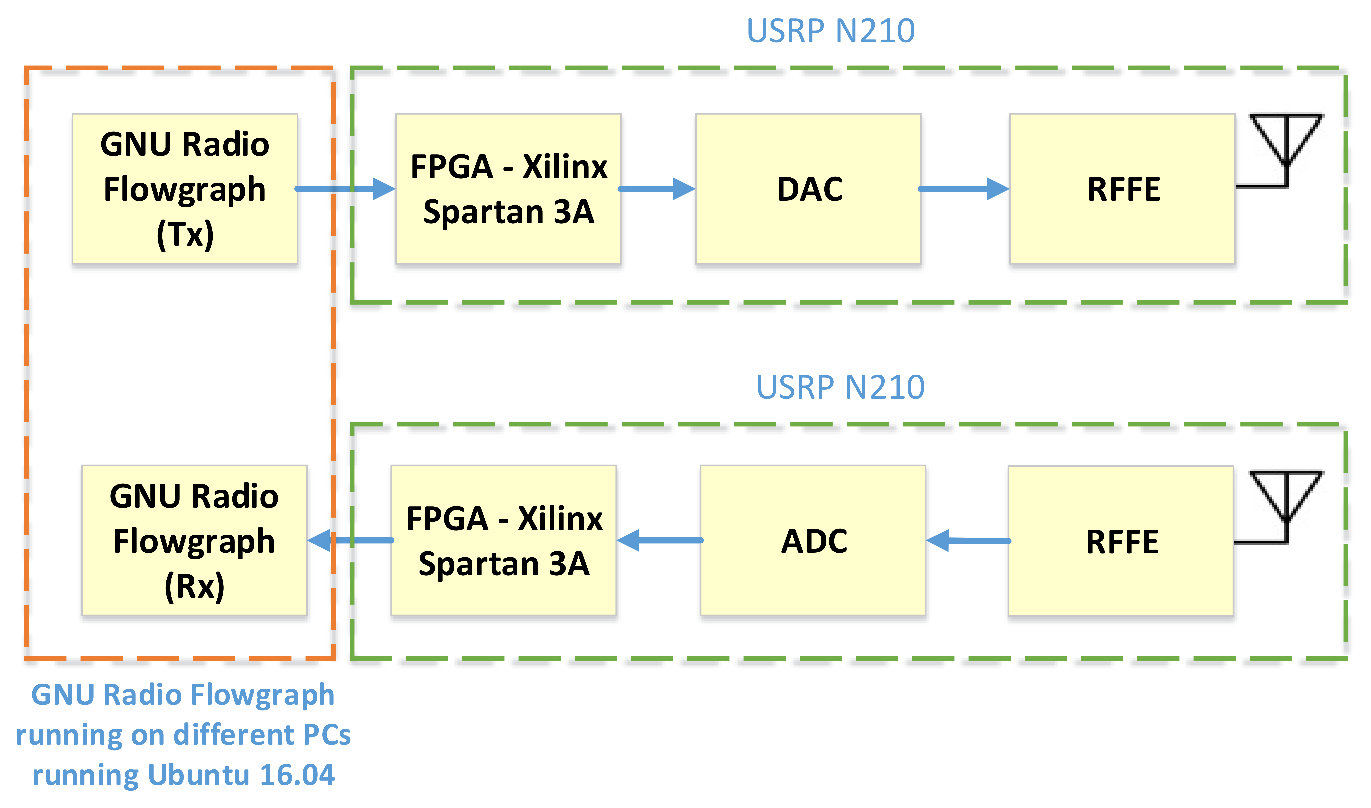
\includegraphics[width=\textwidth,keepaspectratio]{images/Gill/figs/gnuradio.eps}
    \caption{GNURadio and Software-Defined Radio} 
\label{gnuradio}      
\end{figure}

GNU Radio provides a very structured framework of flow design. Data processing segments are extremely self contained to minimize error propagation during system debugging.
Since the software is open-source full access to all code is provide, giving low-level access to all operation within GNU Radio. Much of the actions have been abstracted to limited the
knowledge of the lower layers, but if specific actions are required for an application. Then serious depth or knowledge is needed about the overall project’s structure, which is quite
overloading.[Travisthesis]

\subsection{MATLAB}
MATLAB is an extremely well known engineering, mathematical, biological, and financial software suite. MATLAB provide massive data leverage and advanced communication
system models and algorithm for significant data processing. Since 2007, they have also provided hardware compliance with specific SDR platforms through their Simulink plat-
form, and more recently within MATLAB itself [47]. This thesis primarily utilizes the signal processing and communication system aspects of MATLAB, since MATLAB cannot
fully utilize all aspects of the chosen hardware. It is important to note under alternate constraints, MATLAB can provide adequate performance directly interfacing with hard-
ware, especially when accessing its targeting features seen here [48]. Figure 2.10 shows an example of a common MATLAB SDR model through Simulink.[Travis]


\section{Summary}
This chapter outlined and examined the topics of jamming and anti-jamming techniques, and provided a foundation in communication system theory and advanced equalizer design.  Secondly it setup an understanding of Software-Defined Radio, the power of such an architecture, and examples of implementations and existing software for future designs.  Next, this thesis will consider a new anti-jamming technique and design an implementation of such a system.  After the implementation is investigated, the result of specific experiments on such an implementation will be analyzed.\\
